\section{Experiment 3}

\subsection{Theoretical Backround}

The goal of this mini-experiment to measure basic kinematics with the assuption of constant velocity/acceleration between two points of measurement. Under this prerequisite we can use the basic formulas
\begin{equation}
    v = \frac{\Delta x}{\Delta t}
\end{equation}
\noindent
and
\begin{equation}
    a = \frac{\Delta v}{\Delta t}
\end{equation}
\noindent
to calculate the corresponding quantities.\\
In order to measure those variables in our experiment we use the \texttt{HC-SR04 Ultrasonic sensor}.\\
The Sensor emmits sound waves and notices their arrival of them after being reflected by the surroundings and returns the time difference between those two events, which we use to analyse our distances and kinematics.\\

\subsection{Execution}

\begin{figure}[H]
    \centering
    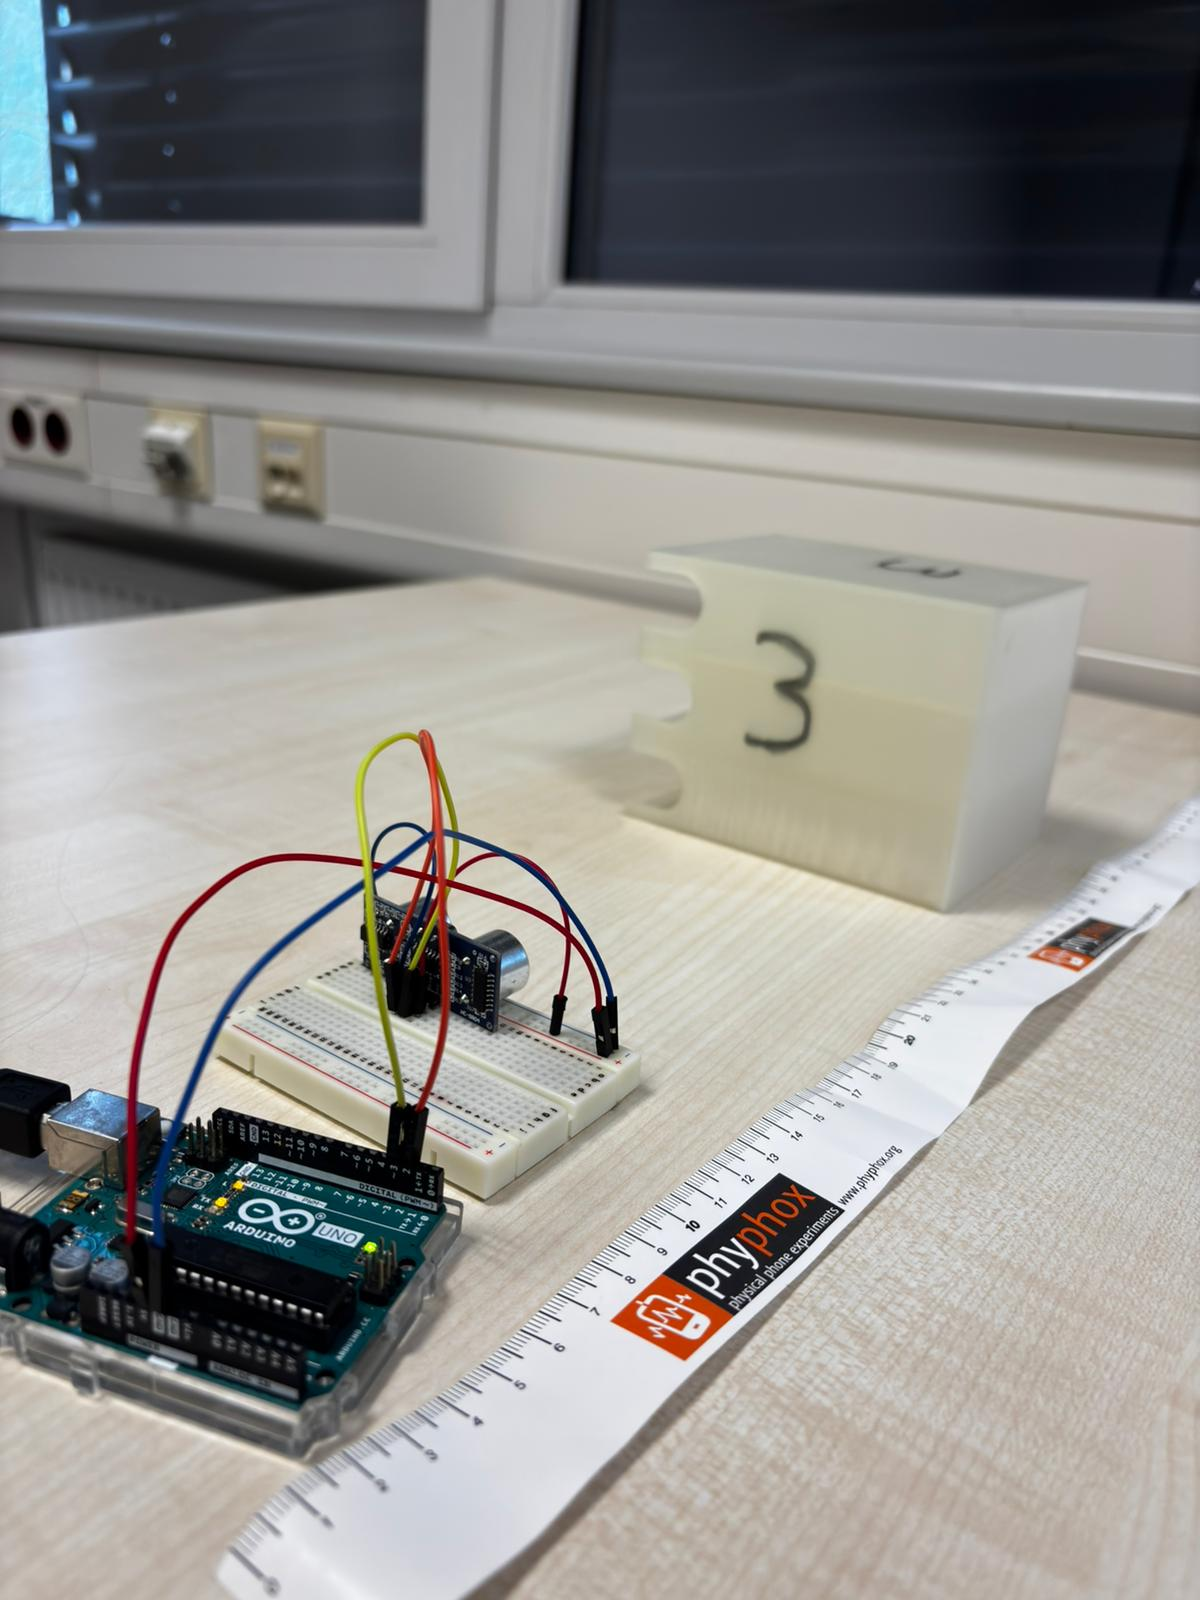
\includegraphics[height=5cm]{../temp_figures/exp3/exp3_1.jpg}
    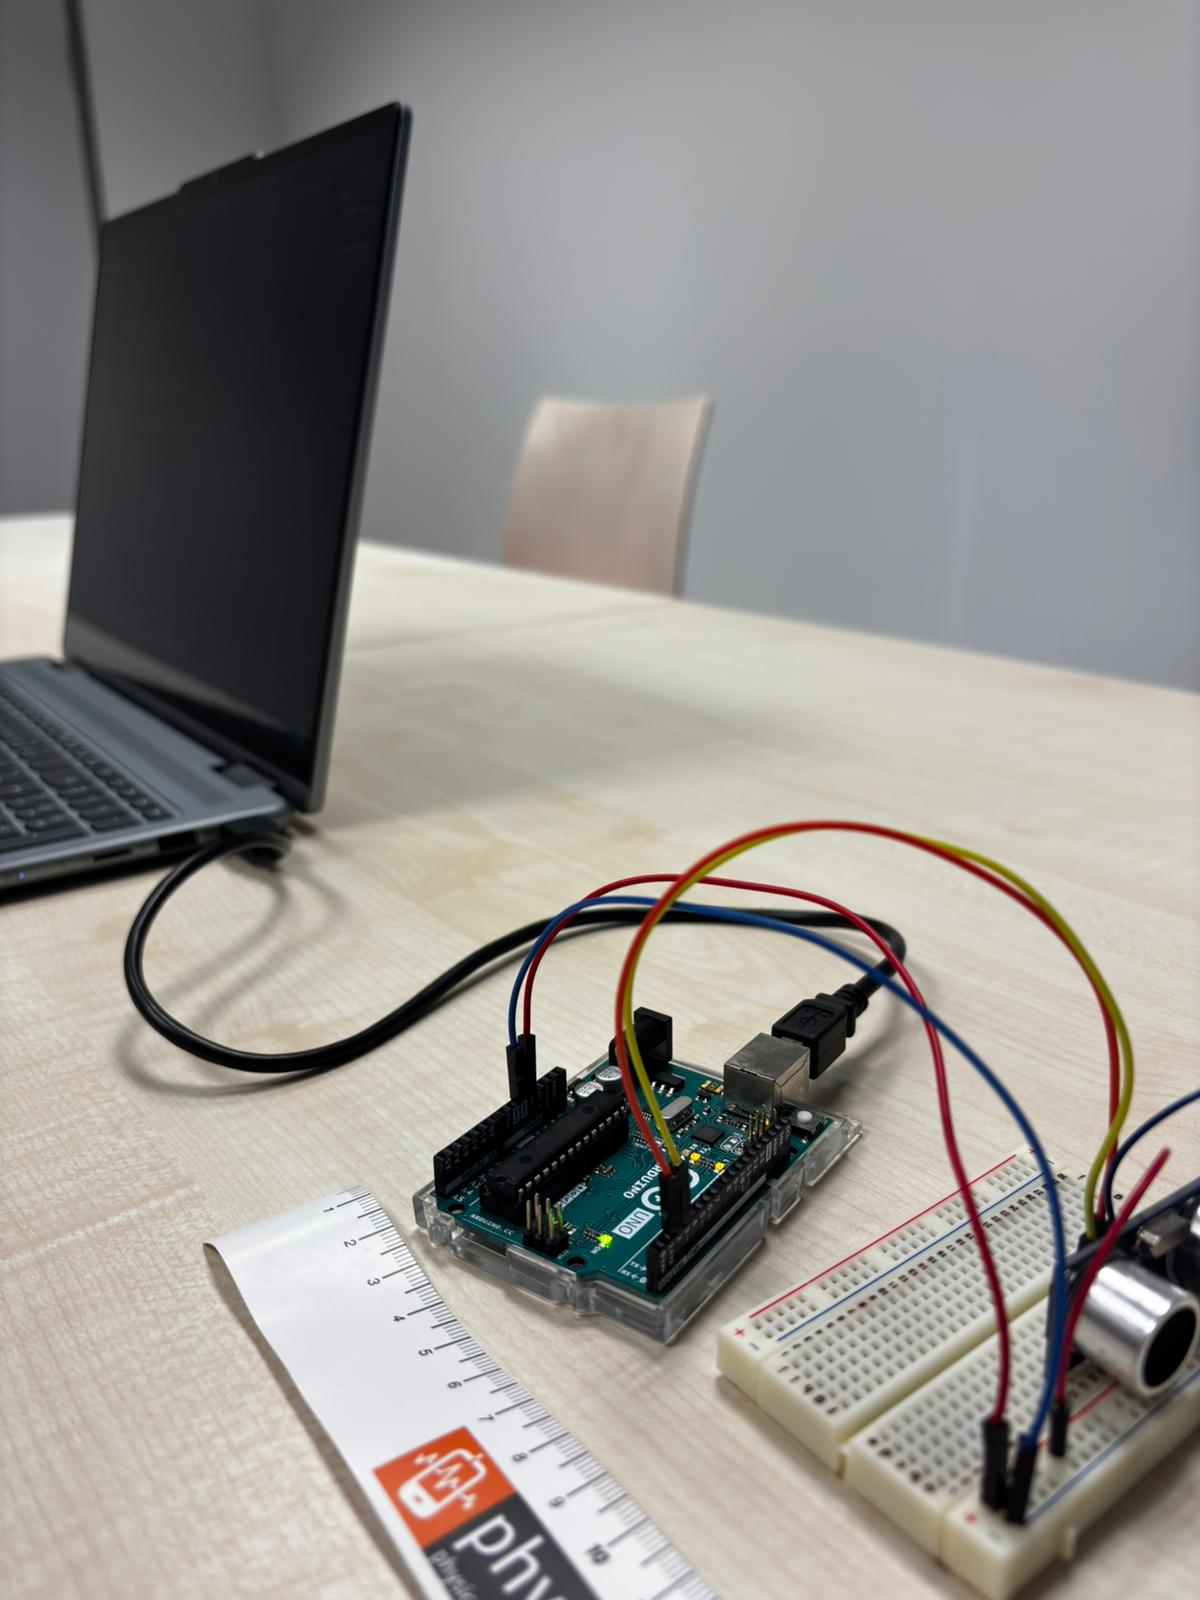
\includegraphics[height=5cm]{../temp_figures/exp3/exp3_2.jpg}
    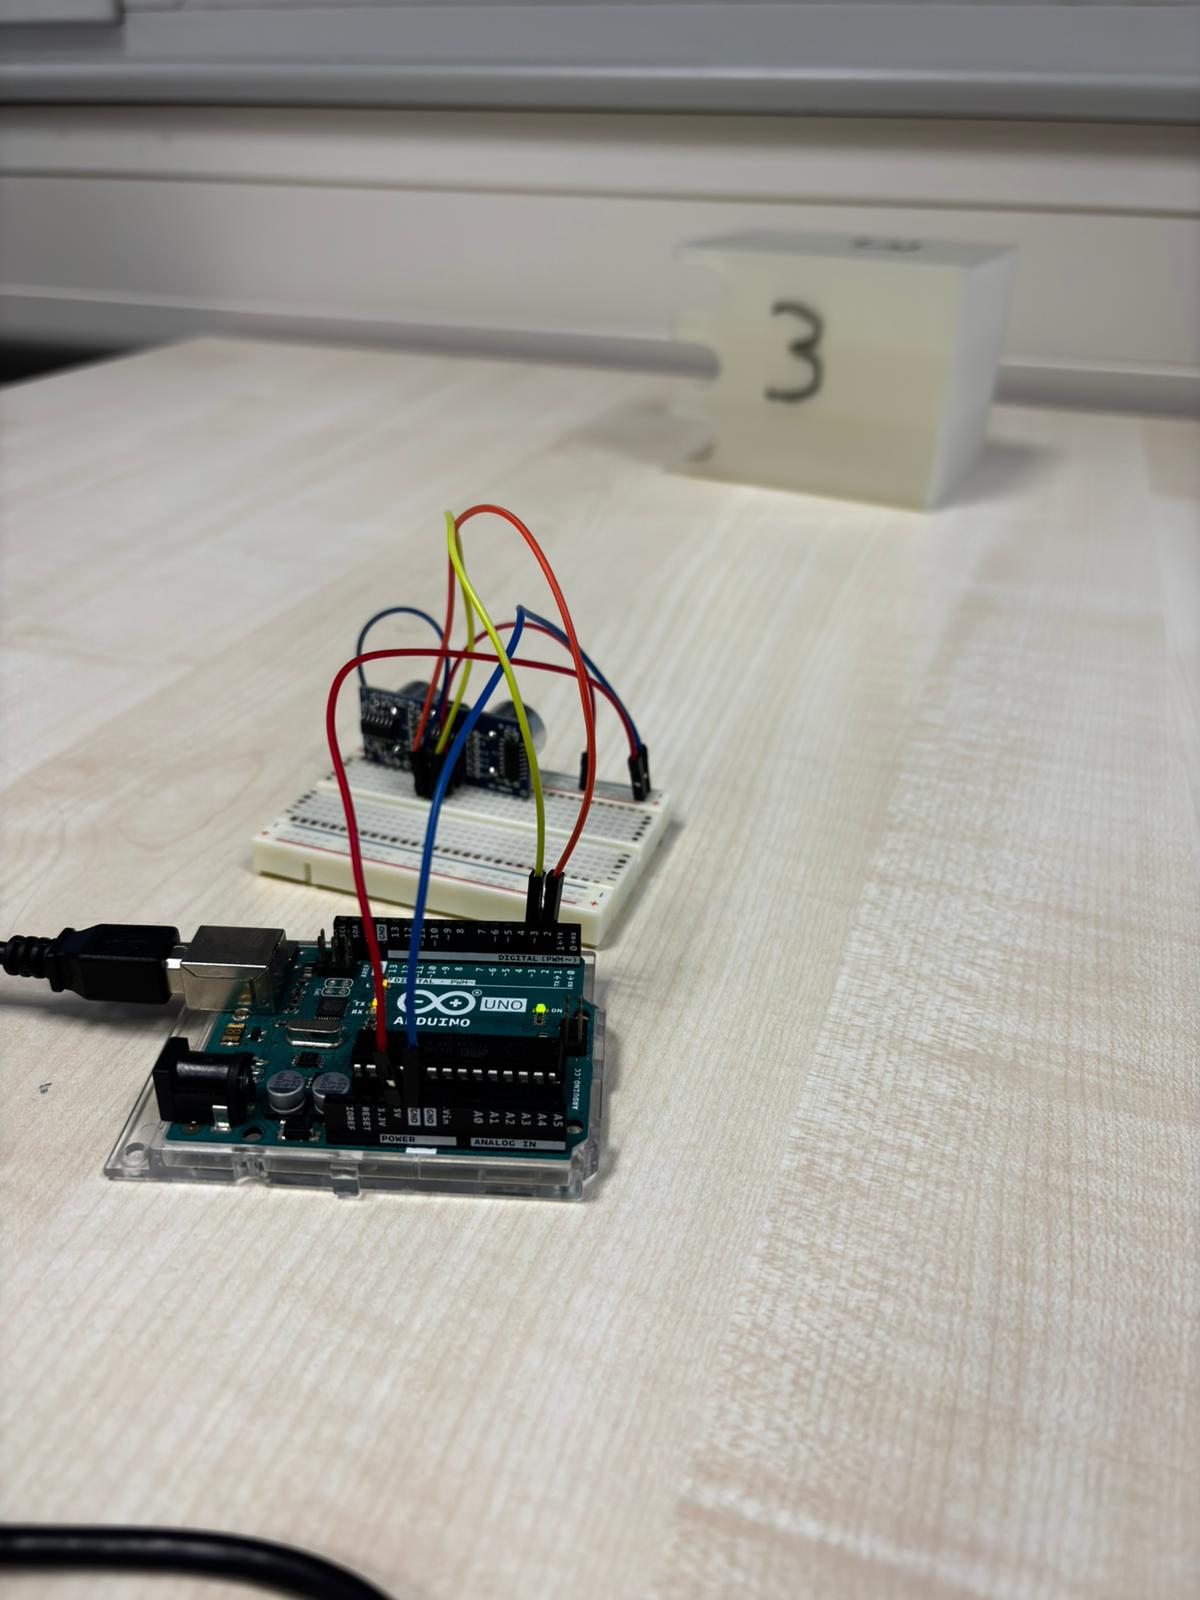
\includegraphics[height=5cm]{../temp_figures/exp3/exp3_3.jpg}
    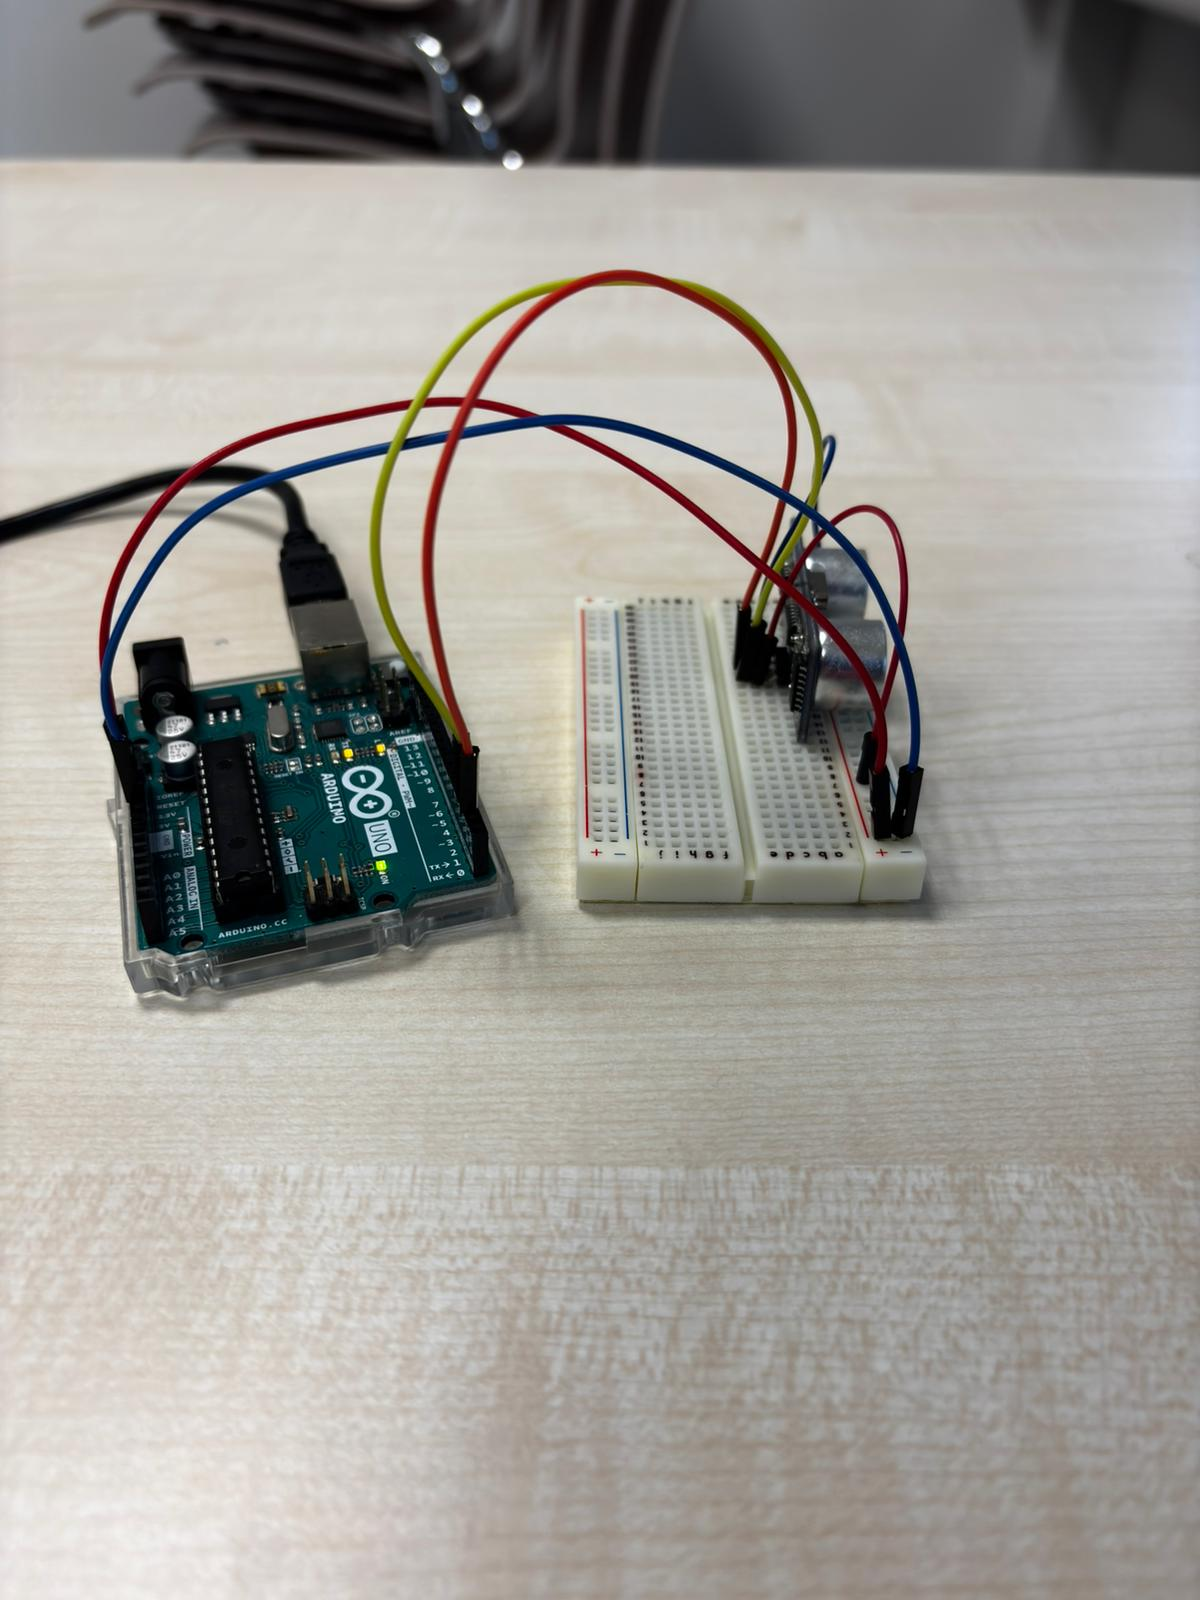
\includegraphics[height=5cm]{../temp_figures/exp3/exp3_4.jpg}
    \caption{Pictures of the set up}
    \label{exp3picture}
\end{figure}

Using the set up as described in the instruction, we connected the sensor to the \texttt{Arduino Uno} and controlled it with our Laptop. To read the sensor we used the code
\inputminted[bgcolor=lightgray]{c}{../experiments/exp3/arduino/3_sketch.ino}
\noindent
and to read the Arduino and save the data we used the code
\inputminted[bgcolor=lightgray]{c}{../experiments/exp3/python/3.py}
\noindent
only changing the according output file names in between the measurements. The time of the measurements was controlled manually.

\subsection{Results}

Assuming a speed of light of $340 \unit{\frac{\meter}{\second}}$, the manufactorer states a resolution of $0.3 \unit{\centi\meter}$, which we can assume to by our uncertainty. We note, that for all measurements
\begin{equation}
    v_\text{sound} = \frac{2d}{\Delta t}
\end{equation}
\noindent
with the distande $d$ and measured time difference $\Delta t$. Assuming $v_\text{sound}=340 \unit{\frac{\meter}{\second}}$ (no error) we calculate
\begin{equation}
    sigma_t = \frac{2\sigma_d}{v_\text{sound}} = 17.7 \unit{\micro\second}
\end{equation}
\noindent
